%This problem and the next study the heat equation in two dimensions.  
This problem and the next study equations in two dimensions.  
We begin with the steady-state problem.  
In place of the one dimensional equation, $-u'' = f$, we now have
\[ \hspace*{10em}-(u_{xx}(x,y) +u_{yy}(x,y)) = f(x,y), 
   \qquad 0\le x \le 1, \quad 0\le y\le 1,\]
with homogeneous Dirichlet boundary conditions $u(x,0)=u(x,1)=u(0,y)=u(1,y)=0$ 
for all $0\le x\le 1$ and $0\le y\le 1$.
The associated operator $L$ is defined as
\[ L u = -(u_{xx} + u_{yy}),\]
acting on the space $C^2_D[0,1]^2$ consisting of twice continuously differentiable 
functions on $[0,1]\times[0,1]$ with homogeneous boundary conditions.
We can solve the differential equation $Lu=f$ using the spectral method just as we
have seen in class before.
This problem will walk you through the process;  
you may consult Section~8.2 of the text for hints.

\begin{enumerate}
\item Show that $L$ is symmetric, given the inner product 
        \[ (v, w) = \int_0^1 \int_0^1 v(x,y) w(x,y) \, dx@@ dy.\]

\vspace*{0.5em}
\item Verify that the functions 
               \[ \psi_{j,k}(x,y) = 2 \sin(j \pi x) \sin(k \pi y)\]
      are eigenfunctions of $L$ for $j,k = 1,2,\ldots.$\\
      (To do this, you simply need to show that $L\psi_{j,k} = \lambda_{j,k} \psi_{j,k}$
       for some scalar $\lambda_{j,k}$.)  
       
       What is the eigenvalue $\lambda_{j,k}$ associated with $\psi_{j,k}$?

\vspace*{0.5em}
\item Compute the inner product $(\psi_{j,k},\psi_{j,k}) = \norm{\psi_{j,k}}^2$.

\vspace*{0.5em}
\item Let $f(x,y) = x(1-y)$.  Compute the inner product $(f, \psi_{j,k})$.

\vspace*{0.5em}
\item The solution to the diffusion equation is given by the spectral method, but now with
      a double sum to account for all the eigenvalues:
       \[ u(x,y) = \sum_{j=1}^N \sum_{k=1}^N 
                     {1\over \lambda_{j,k}} {(f,\psi_{j,k}) \over (\psi_{j,k},\psi_{j,k})}\, \psi_{j,k}(x,y).\]
      In MATLAB plot the partial sum
       \[ u_{10}(x,y)= \sum_{j=1}^{10} \sum_{k=1}^{10}
                 {1\over \lambda_{j,k}} {(f,\psi_{j,k}) \over (\psi_{j,k},\psi_{j,k})}\, \psi_{j,k}(x,y).\]
      Hint for 3d plots: To plot 
      $\psi_{1,1}(x,y) = 2 \sin(\pi x)\sin(\pi y)$, you could use\\[0em]

       \ \ \ \ \ \ {\tt x = linspace(0,1,40); y = linspace(0,1,40); }

       \ \ \ \ \ \ {\tt [X,Y] = meshgrid(x,y);}

       \ \ \ \ \ \ {\tt Psi11 = 2*sin(pi*X).*sin(pi*Y);}
       
       \ \ \ \ \ \ {\tt surf(X,Y,Psi11)}

\end{enumerate}


%%%%%%%%%%%%%%%%%%%%%%%%%%%%%%%%%%%%%%%%%%%%%%%%%%%%%%%%%%%%%%%%%%%%%%%%%%%%%%%%

\ifthenelse{\boolean{showsols}}{\begin{solution}
\begin{enumerate}
\item To show that $L$ is symmetric, we must show that $(Lu,v) = (u,Lv)$ 
for all $u,v \in C^2_D[0,1]^2$.
We can establish this result by integrating by parts twice in each spatial dimension:
\begin{eqnarray*}
 (Lu,v) &=& -\int_0^1 \int_0^1 \big(u_{xx}(x,y)+u_{yy}(x,y)\big) v(x,y)\,\dop x\,\dop y  \\[0.5em]
        &=& -\int_0^1 \Big(\int_0^1 u_{xx}(x,y)v(x,y)\,\dop x\Big)\,\dop y  
            -\int_0^1 \Big(\int_0^1 u_{yy}(x,y)v(x,y)\,\dop y\Big)\,\dop x  \\[1em]
        &=& \int_0^1 \Big(-\Big[u_x(x,y) v(x,y)\Big]_{x=0}^1 
                          +\Big[u(x,y) v_x(x,y)\Big]_{x=0}^1 
                          - \int_0^1 u(x,y)v_{xx}(x,y)\,\dop x\Big)\,\dop y  \\[0.5em]
        && {} +\int_0^1 \Big(-\Big[u_y(x,y) v(x,y)\Big]_{y=0}^1 
                          +\Big[u(x,y) v_y(x,y)\Big]_{y=0}^1 
                          - \int_0^1 u(x,y)v_{yy}(x,y)\,\dop y\Big)\,\dop x \\[1em] 
        &=& -\int_0^1 \Big(\int_0^1 u(x,y)v_{xx}(x,y)\,\dop x\Big)\,\dop y  
            -\int_0^1 \Big(\int_0^1 u(x,y)v_{yy}(x,y)\,\dop y\Big)\,\dop x  \\[1em]
        &=& -\int_0^1 \int_0^1 u(x,y)\big(v_{xx}(x,y)+v_{yy}(x,y)\big)\,\dop x\,\dop y  \\[1em]
        &=& (u,Lv).
\end{eqnarray*}
More generally, you can appeal to Green's Second Identity, which amounts to 
integration by parts in higher dimensions.  Let $\Omega:= [0,1]\times [0,1]\subset \R^2$
denote the domain $0\le x\le 1$ and $0\le y\le 1$, and $\partial \Omega$ its boundary.
We write $-Lu = -u_{xx}-u_{yy} = -\Delta u$.
Green's Second Identity gives
\[ \int_\Omega \big((\Delta u) v - u (\Delta v)\big) \,\dop V
     = \int_{\partial \Omega} \Big( u {\partial v\over \partial n} - v{\partial u\over \partial n}\Big)\,\dop S,\]
where $\partial u/\partial n$ and $\partial v/\partial n$ denote derivatives with respect
to the outward-pointing normal direction.
Thus
\[ (Lu,v) = -\int_\Omega (\Delta u) v\, dV 
          = -\int_\Omega  u (\Delta v)\, dV
          +\int_{\partial \Omega} \Big( u {\partial v\over \partial n} - v{\partial u\over \partial n}\Big)\,\dop S
          = -\int_\Omega  u (\Delta v)\, dV
          = (u,Lv),\]
since $u$ and $v$ are zero on the boundary $\partial \Omega$.


\item We simply compute
        \begin{eqnarray*}
          L \psi_{j,k}  = 
                    -\Big({\d^2\psi_{j,k} \over \d x^2}  
                        + {\d^2\psi_{j,k} \over \d y^2}\Big)
           &=& -{\d \over \d x^2} (\sin(j\pi x)\sin(k\pi y)
             -{\d \over \d y^2} (\sin(j\pi x)\sin(k\pi y) \\[0.5em]
           &=& j^2\pi^2 \sin(j\pi x)\sin(k\pi y)
             + k^2 \pi^2 \sin(j\pi x)\sin(k\pi y) \\[0.5em]
           &=& (j^2 + k^2)\pi^2 \sin(j\pi x)\sin(k\pi y) \\[0.5em]
           &=& \lambda_{j,k} \psi_{j,k}(x,y).
        \end{eqnarray*} 
      One can also notice that $\psi_{j,k}(x,y)$ satisfies the
      necessary boundary conditions 
         \[ \psi_{j,k}(0,y) = \psi_{j,k}(1,y) 
                            = \psi_{j,k}(x,0) = \psi_{j,k}(x,1) = 0.\]
      {[GRADERS: please deduct 2 points if the student forgot 
                to check the boundary conditions.]}

      Thus $\psi_{j,k}(x,y) = \sin(j\pi x)\sin(k\pi x)$ is an 
      eigenfunction for the operator $L$.

\item The computation in part~(b) reveals the eigenvalue to be 
       $\lambda_{j,k}=(j^2+k^2)\pi^2$.

\item The inner product computation reduces to the product of 
      single integrals:
      \begin{eqnarray*}
           (\psi_{j,k}, \psi_{j,k}) 
              &=& 4\int_0^1 \int_0^1 \sin(j\pi x)^2 \sin(k\pi y)^2\, dx\,dy \\[0.5em]
              &=& 4\Big(\int_0^1 \sin(j\pi x)^2\, dx \Big)
                  \Big(\int_0^1 \sin(k\pi y)^2\, dy \Big) \\[0.5em]
              &=& 1.
      \end{eqnarray*}

\item This inner product also breaks into the products of two integrals
         that are straightforward to compute:
      \begin{eqnarray*}
           (f, \psi_{j,k}) 
              &=& 2 \int_0^1 \int_0^1 x(1-y)\sin(j\pi x) \sin(k\pi y)\, dx\,dy \\[0.5em]
              &=& 2 \Big(\int_0^1 x \sin(j\pi x)\, dx \Big)
                  \Big(\int_0^1 (1-y)\sin(k\pi y)^2\, dy \Big) \\[0.5em]
              &=& 2 \Big({(-1)^{j+1}\over j\pi} \Big)
                  \Big({1\over k\pi} \Big) \\[0.5em]
              &=& 2{(-1)^{j+1} \over jk\pi^2}.
      \end{eqnarray*}
    
\item The code below plots the partial sum 
         \[ u_N(x,y) = \sum_{j=1}^N  \sum_{k=1}^N 
                       { (f,\psi_{j,k}) \over \lambda_{j,k} (\psi_{j,k}, \psi_{j,k})}
                       \psi_{j,k}(x,y)\]
      for various values of $N$, as shown in the plots below.

      \begin{center} 
          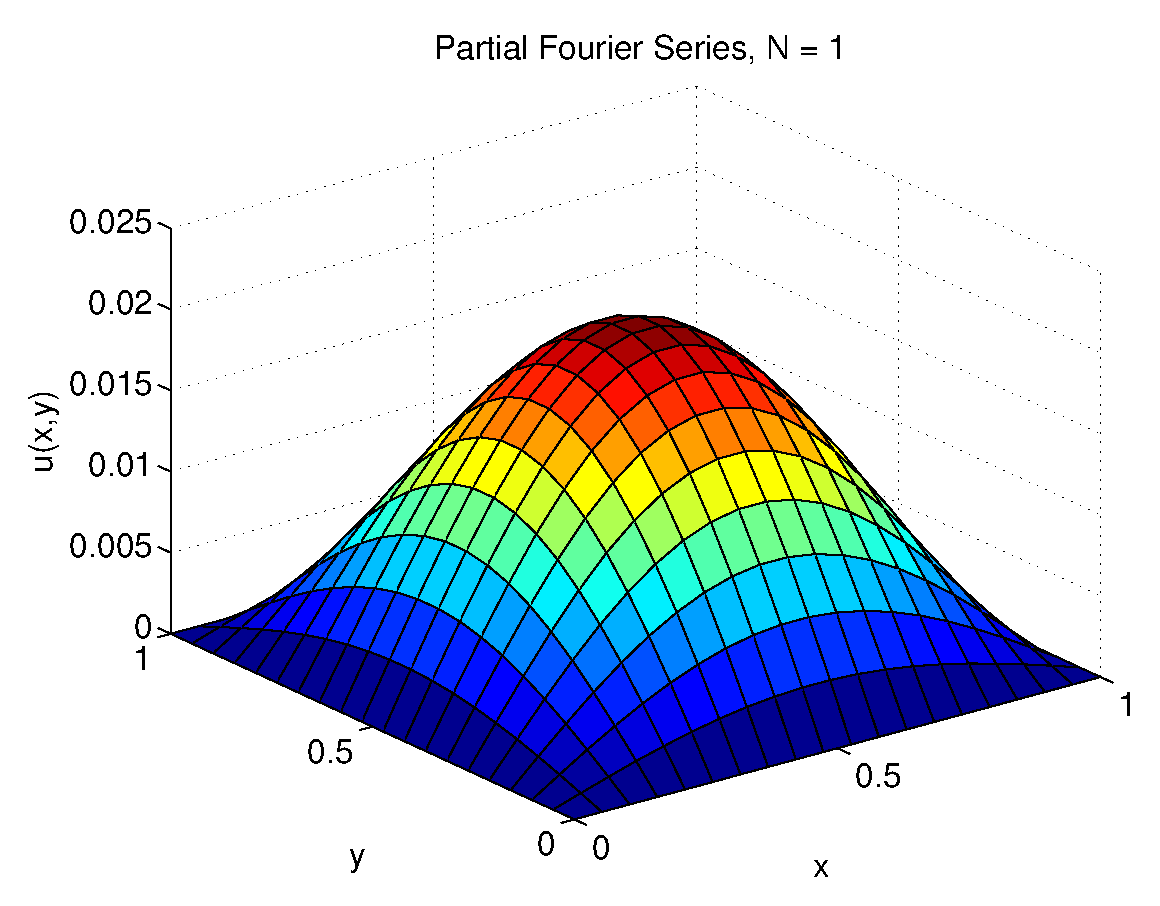
\includegraphics[scale=0.37]{twoD1}\quad
          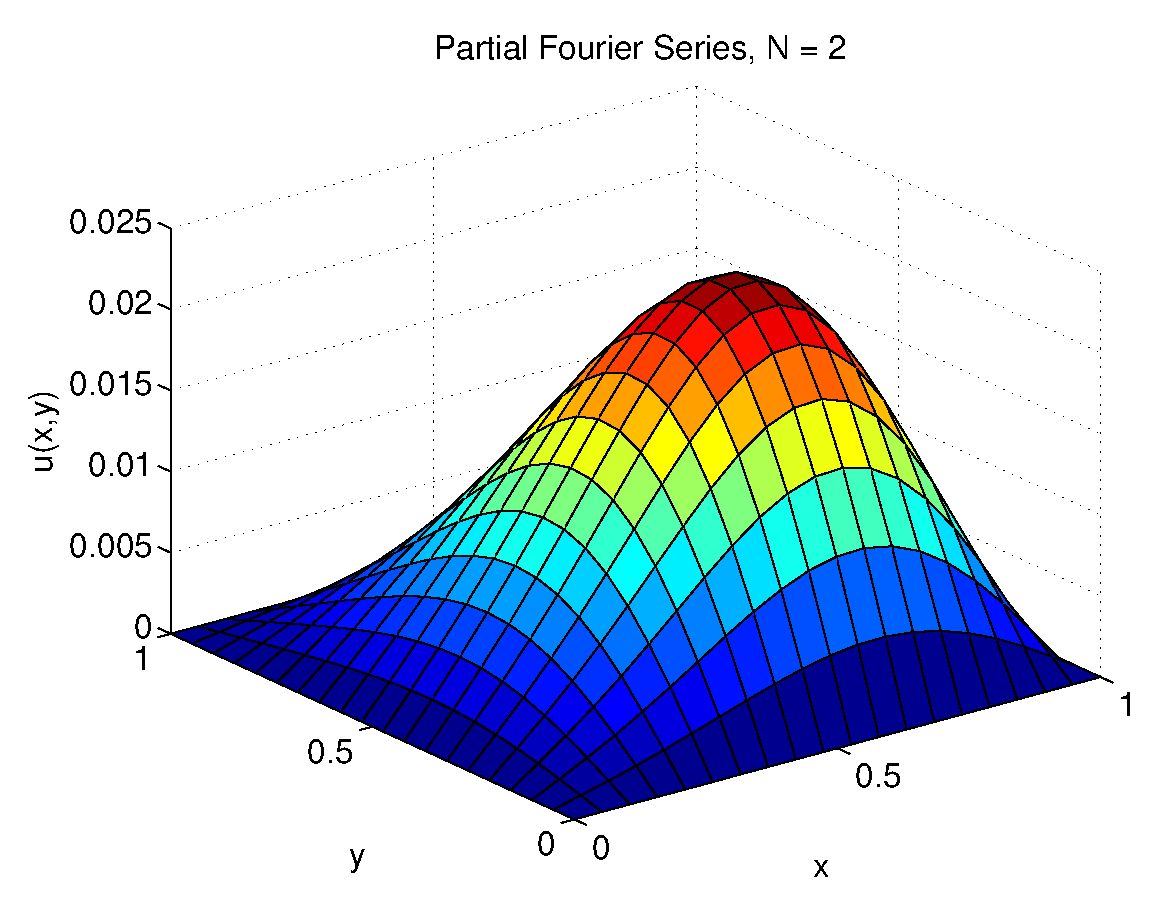
\includegraphics[scale=0.37]{twoD2}

          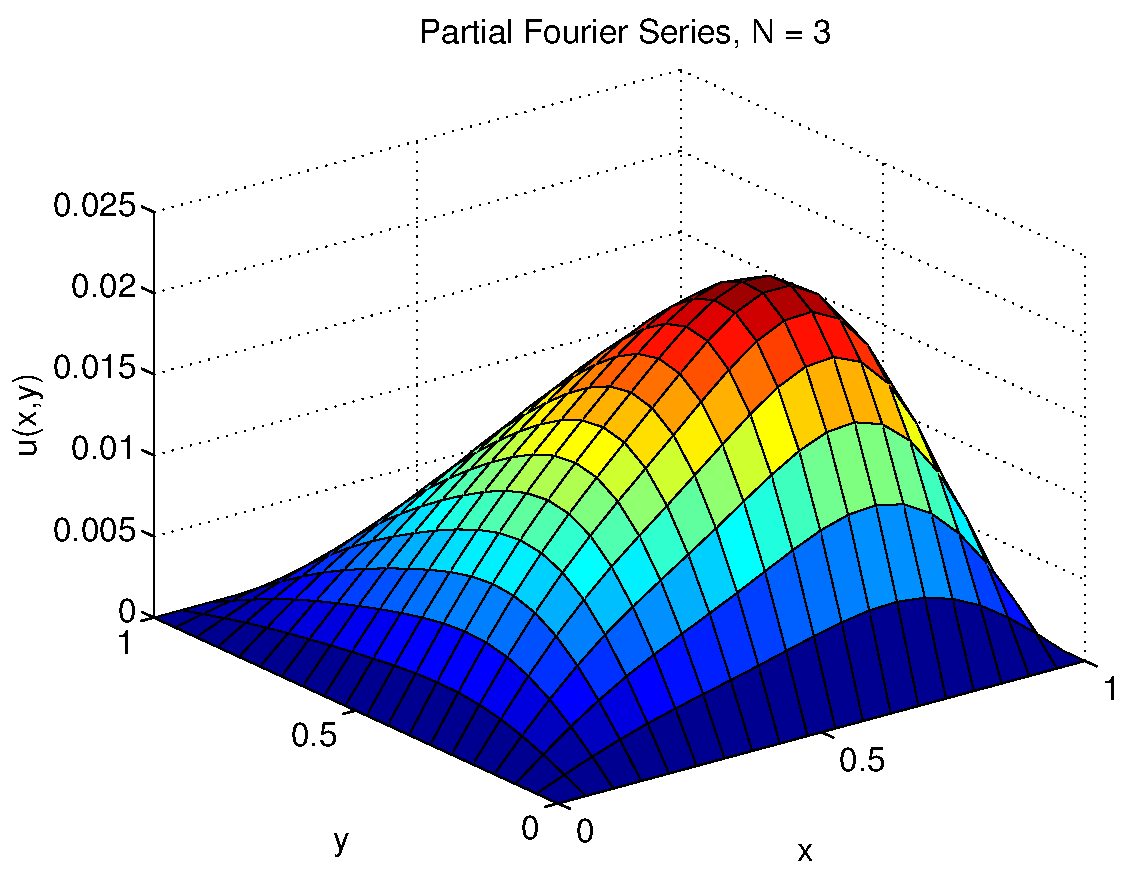
\includegraphics[scale=0.37]{twoD3}\quad
          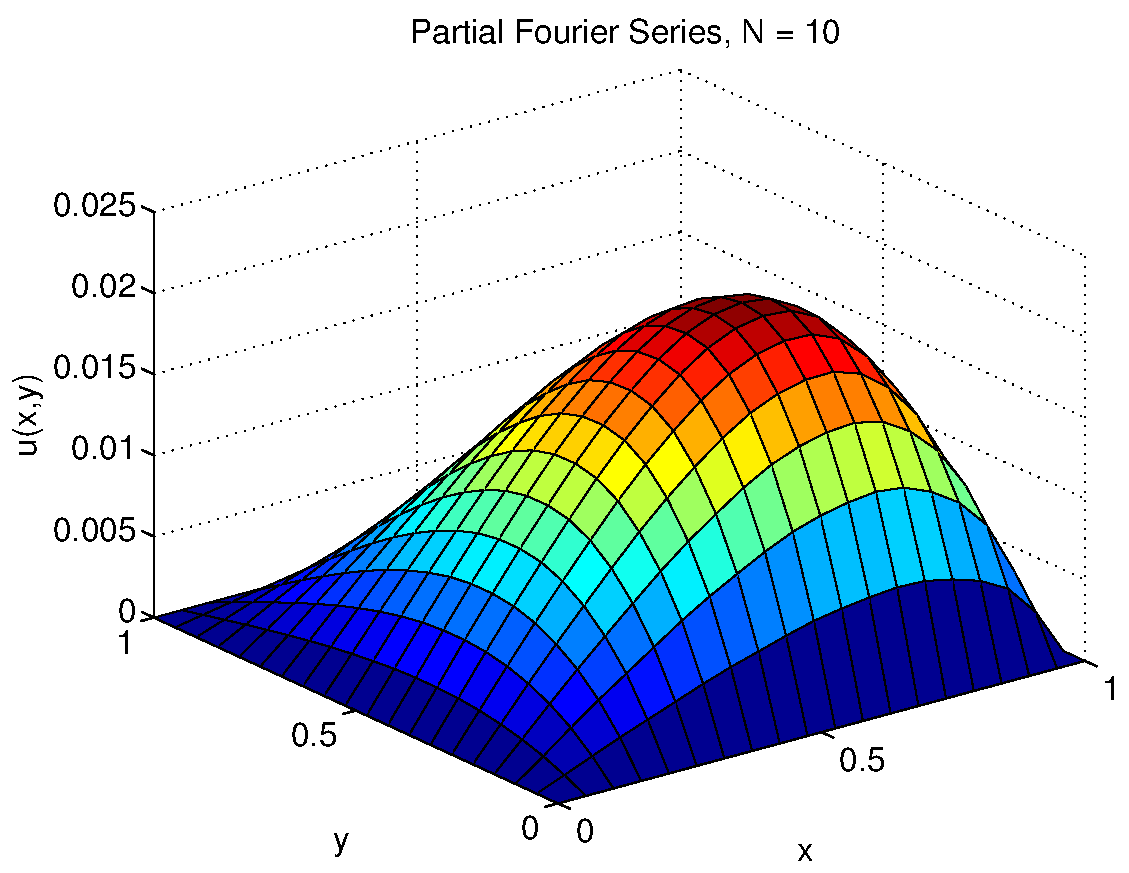
\includegraphics[scale=0.37]{twoD10}
      \end{center}

     \input twoDcode
\end{enumerate}
\end{solution}}{}

